\documentclass[12pt,a4paper]{report}

% ============================================================================
% PACKAGES
% ============================================================================
\usepackage[utf8]{inputenc}
\usepackage[T1]{fontenc}
\usepackage{lmodern}
\usepackage[margin=1in]{geometry}
\usepackage{graphicx}
\usepackage{xcolor}
\usepackage{hyperref}
\usepackage{tikz}
\usepackage{longtable}
\usepackage{booktabs}
\usepackage{fancyhdr}
\usepackage{titlesec}
\usepackage{listings}
\usepackage{enumitem}
\usepackage{tabularx}

% TikZ Libraries
\usetikzlibrary{shapes.geometric, arrows.meta, positioning, fit, backgrounds}

% ============================================================================
% COLORS
% ============================================================================
\definecolor{primaryblue}{RGB}{26, 54, 93}
\definecolor{secondaryblue}{RGB}{59, 130, 246}
\definecolor{accentgreen}{RGB}{34, 197, 94}
\definecolor{warningorange}{RGB}{249, 115, 22}
\definecolor{lightgray}{RGB}{243, 244, 246}
\definecolor{darkgray}{RGB}{75, 85, 99}

% ============================================================================
% HYPERREF SETUP
% ============================================================================
\hypersetup{
    colorlinks=true,
    linkcolor=primaryblue,
    urlcolor=secondaryblue,
    pdftitle={EduX - Student Management Guide},
    pdfauthor={EduX Development Team},
}

% ============================================================================
% HEADER/FOOTER
% ============================================================================
\pagestyle{fancy}
\fancyhf{}
\fancyhead[L]{\textcolor{darkgray}{\small EduX School Management System}}
\fancyhead[R]{\textcolor{darkgray}{\small Student Management Guide}}
\fancyfoot[C]{\textcolor{darkgray}{\thepage}}
\renewcommand{\headrulewidth}{0.4pt}

% ============================================================================
% TITLE FORMATTING
% ============================================================================
\titleformat{\chapter}[display]
  {\normalfont\huge\bfseries\color{primaryblue}}
  {\chaptertitlename\ \thechapter}{20pt}{\Huge}

\titleformat{\section}
  {\normalfont\Large\bfseries\color{primaryblue}}
  {\thesection}{1em}{}

\titleformat{\subsection}
  {\normalfont\large\bfseries\color{secondaryblue}}
  {\thesubsection}{1em}{}

% ============================================================================
% DOCUMENT
% ============================================================================
\begin{document}

% ----------------------------------------------------------------------------
% TITLE PAGE
% ----------------------------------------------------------------------------
\begin{titlepage}
    \centering
    \vspace*{2cm}
    
    {\Huge\bfseries\textcolor{primaryblue}{EduX}\par}
    \vspace{0.5cm}
    {\Large\textcolor{secondaryblue}{School Management System}\par}
    
    \vspace{2cm}
    
    
\begin{tikzpicture}
        \node[draw=primaryblue, line width=2pt, rounded corners=10pt, 
              minimum width=8cm, minimum height=3cm, fill=lightgray] 
              {\Huge\bfseries\textcolor{primaryblue}{Student Management}};
    \end{tikzpicture}
    
    \vfill
    
    {\large\textcolor{darkgray}{Version 1.0}\par}
    {\large\textcolor{darkgray}{\today}\par}
\end{titlepage}

% ----------------------------------------------------------------------------
% TABLE OF CONTENTS
% ----------------------------------------------------------------------------
\tableofcontents
\newpage

% ============================================================================
% CHAPTER 1: OVERVIEW
% ============================================================================
\chapter{Student Management Overview}

\section{Introduction}

The Student Management module is the core of EduX, providing comprehensive tools for managing the complete student lifecycle from admission to graduation.

\section{Student Lifecycle}

\begin{center}
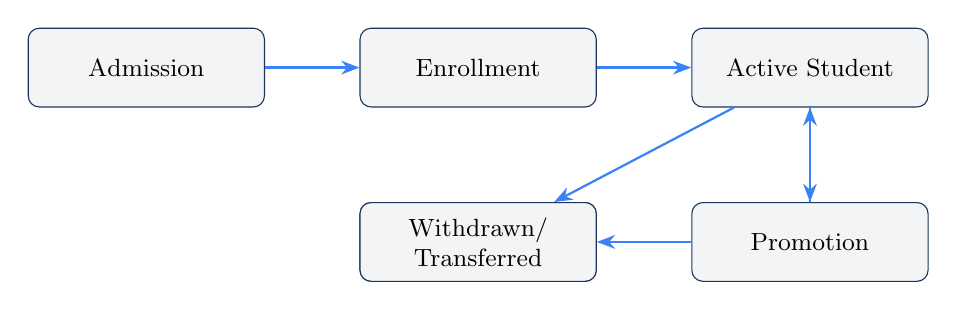
\begin{tikzpicture}[
    node distance=1.2cm,
    state/.style={draw=primaryblue, rounded corners, minimum width=3cm, 
                  minimum height=1cm, fill=lightgray, align=center, font=\small},
    arrow/.style={-{Stealth}, thick, secondaryblue}
]
    \node[state] (admission) {Admission};
    \node[state, right=of admission] (enrollment) {Enrollment};
    \node[state, right=of enrollment] (active) {Active Student};
    \node[state, below=of active] (promotion) {Promotion};
    \node[state, left=of promotion] (graduated) {Graduated};
    \node[state, below=of enrollment] (withdrawal) {Withdrawn/\\Transferred};
    
    \draw[arrow] (admission) -- (enrollment);
    \draw[arrow] (enrollment) -- (active);
    \draw[arrow] (active) -- (promotion);
    \draw[arrow] (promotion) -- (active);
    \draw[arrow] (promotion) -- (graduated);
    \draw[arrow] (active) -- (withdrawal);
\end{tikzpicture}
\end{center}

\section{Student Data Structure}

\begin{center}
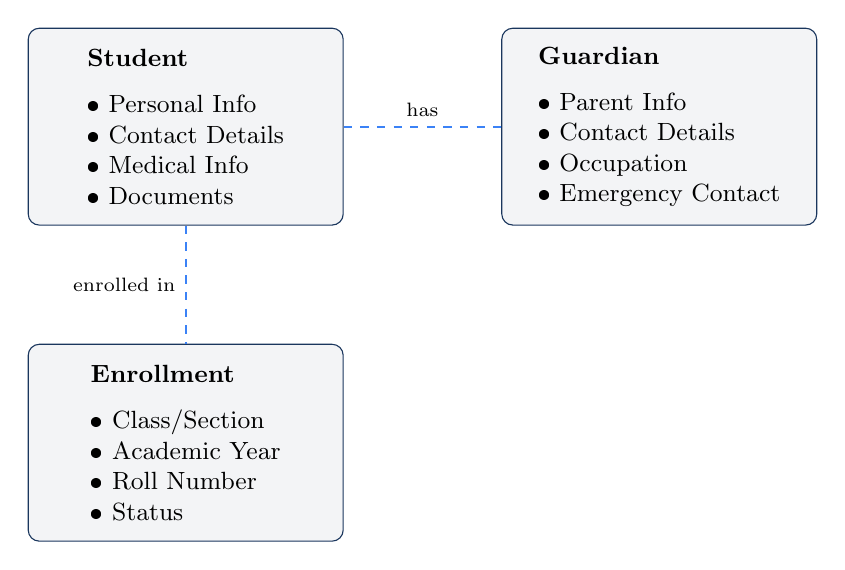
\begin{tikzpicture}[
    entity/.style={draw=primaryblue, rounded corners, minimum width=4cm, 
                   minimum height=2.5cm, fill=lightgray, align=left, font=\small},
    relation/.style={draw=secondaryblue, dashed, thick}
]
    % Student Entity
    \node[entity] (student) at (0,0) {
        \textbf{Student}\\[0.2cm]
        • Personal Info\\
        • Contact Details\\
        • Medical Info\\
        • Documents
    };
    
    % Guardian Entity
    \node[entity, right=2cm of student] (guardian) {
        \textbf{Guardian}\\[0.2cm]
        • Parent Info\\
        • Contact Details\\
        • Occupation\\
        • Emergency Contact
    };
    
    % Enrollment Entity
    \node[entity, below=1.5cm of student] (enrollment) {
        \textbf{Enrollment}\\[0.2cm]
        • Class/Section\\
        • Academic Year\\
        • Roll Number\\
        • Status
    };
    
    % Relations
    \draw[relation] (student) -- node[above, font=\scriptsize] {has} (guardian);
    \draw[relation] (student) -- node[left, font=\scriptsize] {enrolled in} (enrollment);
\end{tikzpicture}
\end{center}

% ============================================================================
% CHAPTER 2: ADDING STUDENTS
% ============================================================================
\chapter{Adding Students}

\section{Add Student Form}

Navigate to \texttt{Students} $\rightarrow$ \texttt{Add Student} to register a new student.

\subsection{Personal Information}

\begin{longtable}{@{}p{4cm}p{3cm}p{6cm}@{}}
\toprule
\textbf{Field} & \textbf{Required} & \textbf{Description} \\
\midrule
\endhead
Admission Number & Yes & Unique identifier (auto-generated or manual) \\
First Name & Yes & Student's first name \\
Last Name & Yes & Student's last name \\
Date of Birth & No & Birth date for age calculation \\
Gender & Yes & Male / Female \\
Blood Group & No & For medical emergencies \\
Religion & No & Student's religion \\
Nationality & No & Default: Pakistani \\
CNIC / B-Form & No & National identity number \\
\bottomrule
\end{longtable}

\subsection{Contact Information}

\begin{longtable}{@{}p{4cm}p{3cm}p{6cm}@{}}
\toprule
\textbf{Field} & \textbf{Required} & \textbf{Description} \\
\midrule
\endhead
Address & No & Residential address \\
City & No & City of residence \\
Phone & No & Contact number \\
Email & No & Email address \\
\bottomrule
\end{longtable}

\subsection{Medical Information}

\begin{longtable}{@{}p{4cm}p{3cm}p{6cm}@{}}
\toprule
\textbf{Field} & \textbf{Required} & \textbf{Description} \\
\midrule
\endhead
Medical Info & No & Any medical conditions \\
Allergies & No & Known allergies \\
Special Needs & No & Learning or physical needs \\
\bottomrule
\end{longtable}

\subsection{Academic Information}

\begin{longtable}{@{}p{4cm}p{3cm}p{6cm}@{}}
\toprule
\textbf{Field} & \textbf{Required} & \textbf{Description} \\
\midrule
\endhead
Class & Yes & Class to enroll in \\
Section & Yes & Section within class \\
Roll Number & No & Roll number in class \\
Admission Date & Yes & Date of admission \\
Previous School & No & Name of previous school \\
\bottomrule
\end{longtable}

\section{Student Photo}

Upload a student photo:
\begin{itemize}[leftmargin=*]
    \item Supported formats: PNG, JPG, JPEG
    \item Recommended size: 300 × 300 pixels
    \item Maximum file size: 2 MB
    \item Click the photo placeholder to upload
\end{itemize}

% ============================================================================
% CHAPTER 3: GUARDIAN MANAGEMENT
% ============================================================================
\chapter{Guardian Management}

\section{Adding Guardians}

Each student can have multiple guardians (parents, relatives, etc.).

\subsection{Guardian Information}

\begin{longtable}{@{}p{4cm}p{3cm}p{6cm}@{}}
\toprule
\textbf{Field} & \textbf{Required} & \textbf{Description} \\
\midrule
\endhead
First Name & Yes & Guardian's first name \\
Last Name & Yes & Guardian's last name \\
Relation & Yes & Father / Mother / Guardian / Other \\
CNIC & No & National identity number \\
Phone & Yes & Primary contact number \\
Alternate Phone & No & Secondary contact \\
Email & No & Email address \\
Occupation & No & Job / Profession \\
Workplace & No & Employer name \\
Address & No & If different from student \\
\bottomrule
\end{longtable}

\subsection{Guardian Flags}

\begin{itemize}[leftmargin=*]
    \item \textbf{Primary Guardian} -- Main contact for communications
    \item \textbf{Can Pickup} -- Authorized to pick up student
    \item \textbf{Emergency Contact} -- Contact in emergencies
\end{itemize}

\section{Multiple Guardians}

\begin{center}
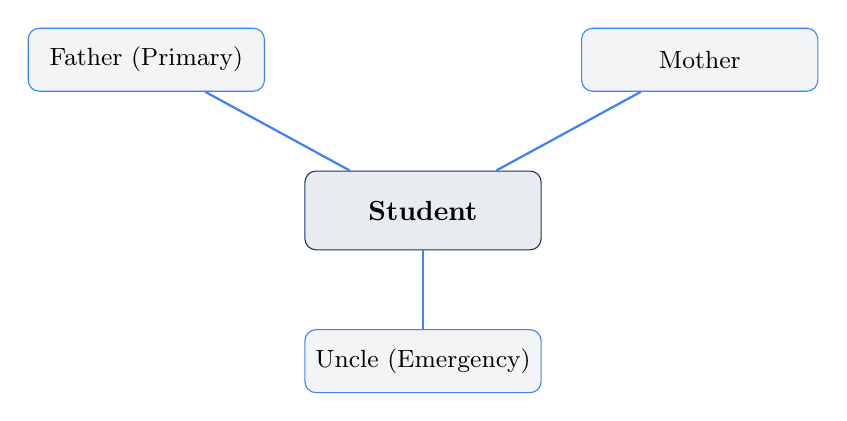
\begin{tikzpicture}[
    node distance=1cm,
    guardian/.style={draw=secondaryblue, rounded corners, minimum width=3cm, 
                     minimum height=0.8cm, fill=lightgray, font=\small},
    student/.style={draw=primaryblue, rounded corners, minimum width=3cm, 
                    minimum height=1cm, fill=primaryblue!10, font=\bfseries},
    line/.style={thick, secondaryblue}
]
    \node[student] (student) {Student};
    \node[guardian, above left=1cm and 0.5cm of student] (father) {Father (Primary)};
    \node[guardian, above right=1cm and 0.5cm of student] (mother) {Mother};
    \node[guardian, below=1cm of student] (uncle) {Uncle (Emergency)};
    
    \draw[line] (student) -- (father);
    \draw[line] (student) -- (mother);
    \draw[line] (student) -- (uncle);
\end{tikzpicture}
\end{center}

% ============================================================================
% CHAPTER 4: STUDENT PROFILES
% ============================================================================
\chapter{Student Profiles}

\section{Viewing Student Profile}

Click on any student in the list to view their complete profile.

\subsection{Profile Sections}

\begin{enumerate}[leftmargin=*]
    \item \textbf{Personal Information} -- Basic details and photo
    \item \textbf{Contact Details} -- Address and phone numbers
    \item \textbf{Guardian Information} -- All linked guardians
    \item \textbf{Enrollment History} -- Class history across years
    \item \textbf{Attendance Summary} -- Attendance percentage
    \item \textbf{Fee Summary} -- Outstanding and paid amounts
    \item \textbf{Exam Results} -- Academic performance
\end{enumerate}

\section{Quick Actions}

From the student profile, you can:

\begin{itemize}[leftmargin=*]
    \item \textbf{Edit} -- Modify student information
    \item \textbf{View Attendance} -- See detailed attendance records
    \item \textbf{View Fees} -- Check fee status and history
    \item \textbf{View Report Card} -- Access academic reports
    \item \textbf{Print ID Card} -- Generate student ID card
    \item \textbf{Transfer/Withdraw} -- Change student status
\end{itemize}

% ============================================================================
% CHAPTER 5: ENROLLMENT MANAGEMENT
% ============================================================================
\chapter{Enrollment Management}

\section{Understanding Enrollments}

Enrollments link students to classes for specific academic years. A student can have multiple enrollment records over time.

\section{Enrollment Workflow}

\begin{center}
\begin{tikzpicture}[
    node distance=0.8cm,
    step/.style={draw=accentgreen, rounded corners, minimum width=5cm, 
                 minimum height=1cm, fill=lightgray, align=center, font=\small},
    arrow/.style={-{Stealth}, thick, accentgreen}
]
    \node[step] (s1) {New Admission};
    \node[step, below=of s1] (s2) {First Enrollment Created};
    \node[step, below=of s2] (s3) {Academic Year Ends};
    \node[step, below=of s3] (s4) {Promotion / Retention};
    \node[step, below=of s4] (s5) {New Enrollment Created};
    
    \draw[arrow] (s1) -- (s2);
    \draw[arrow] (s2) -- (s3);
    \draw[arrow] (s3) -- (s4);
    \draw[arrow] (s4) -- (s5);
\end{tikzpicture}
\end{center}

\section{Enrollment Status}

\begin{longtable}{@{}p{3cm}p{10cm}@{}}
\toprule
\textbf{Status} & \textbf{Description} \\
\midrule
\endhead
Active & Currently enrolled and attending \\
Promoted & Moved to next class \\
Retained & Repeating current class \\
Transferred & Moved to another school \\
Withdrawn & Left school (other reasons) \\
\bottomrule
\end{longtable}

% ============================================================================
% CHAPTER 6: BULK OPERATIONS
% ============================================================================
\chapter{Bulk Operations}

\section{Bulk Import}

Import multiple students from Excel:

\begin{enumerate}[leftmargin=*]
    \item Go to \texttt{Students} $\rightarrow$ \texttt{Import}
    \item Download the template Excel file
    \item Fill in student data following the template
    \item Upload the completed file
    \item Review import preview
    \item Confirm import
\end{enumerate}

\subsection{Import Template Columns}

\begin{lstlisting}[basicstyle=\ttfamily\footnotesize]
admission_number, first_name, last_name, gender, 
date_of_birth, class, section, guardian_name, 
guardian_phone, guardian_relation, address
\end{lstlisting}

\section{Bulk Export}

Export student data:

\begin{enumerate}[leftmargin=*]
    \item Go to \texttt{Students} $\rightarrow$ \texttt{Export}
    \item Select export format (Excel / PDF)
    \item Choose fields to include
    \item Apply filters (class, section, status)
    \item Click \texttt{Export}
\end{enumerate}

\section{Bulk Promotion}

At the end of academic year:

\begin{enumerate}[leftmargin=*]
    \item Go to \texttt{Students} $\rightarrow$ \texttt{Promotion}
    \item Select source class and section
    \item Choose destination class
    \item Select students to promote
    \item Review and confirm
\end{enumerate}

% ============================================================================
% CHAPTER 7: SEARCH AND FILTER
% ============================================================================
\chapter{Search and Filter}

\section{Quick Search}

Use the search bar at the top of the Students screen to search by:
\begin{itemize}[leftmargin=*]
    \item Student name
    \item Admission number
    \item Guardian name
    \item Phone number
\end{itemize}

\section{Advanced Filters}

\begin{longtable}{@{}p{3cm}p{10cm}@{}}
\toprule
\textbf{Filter} & \textbf{Options} \\
\midrule
\endhead
Class & All classes or specific class \\
Section & All sections or specific section \\
Status & Active, Inactive, Graduated, Withdrawn, Transferred \\
Gender & Male, Female, All \\
Academic Year & Current or previous years \\
\bottomrule
\end{longtable}

% ============================================================================
% CHAPTER 8: STUDENT STATUSES
% ============================================================================
\chapter{Student Statuses}

\section{Status Definitions}

\begin{center}
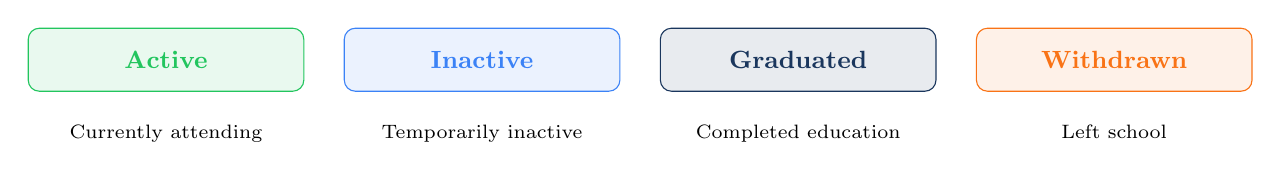
\begin{tikzpicture}[
    status/.style={draw=#1, rounded corners, minimum width=3.5cm, 
                   minimum height=0.8cm, fill=#1!10, font=\small\bfseries, 
                   text=#1},
]
    \node[status=accentgreen] (active) at (0,0) {Active};
    \node[status=secondaryblue, right=0.5cm of active] (inactive) {Inactive};
    \node[status=primaryblue, right=0.5cm of inactive] (graduated) {Graduated};
    \node[status=warningorange, right=0.5cm of graduated] (withdrawn) {Withdrawn};
    
    \node[below=0.3cm of active, font=\scriptsize, text width=3cm, align=center] 
        {Currently attending};
    \node[below=0.3cm of inactive, font=\scriptsize, text width=3cm, align=center] 
        {Temporarily inactive};
    \node[below=0.3cm of graduated, font=\scriptsize, text width=3cm, align=center] 
        {Completed education};
    \node[below=0.3cm of withdrawn, font=\scriptsize, text width=3cm, align=center] 
        {Left school};
\end{tikzpicture}
\end{center}

\section{Changing Student Status}

\begin{enumerate}[leftmargin=*]
    \item Open student profile
    \item Click \texttt{Change Status}
    \item Select new status
    \item Enter leaving date (if applicable)
    \item Provide reason for change
    \item Confirm change
\end{enumerate}

\textbf{Note:} Status changes are logged in the activity history for audit purposes.

\end{document}
